\documentclass{homework}

\input{particulars}

\sisetup{round-precision=3}

\begin{document}

\title{Video Compression HW2}
\author{\chineseName \masterStudentID}
\date{}
\maketitle

I split the image to 8x8 blocks to speed up DCT.

The following images are the result of the coefficients in the log domain.

\begin{figure}[H]
    \centering
    \begin{subfigure}{0.32\textwidth}
        \centering
        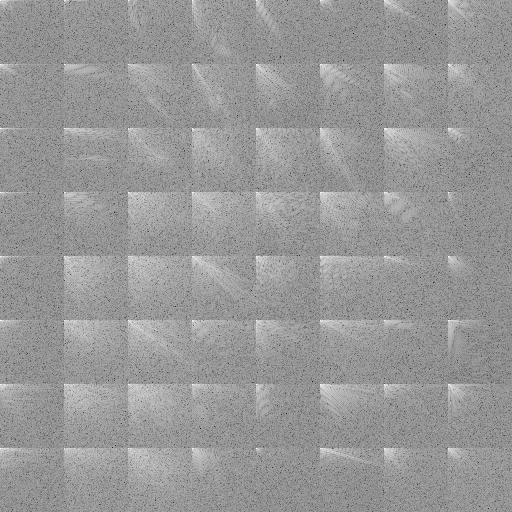
\includegraphics[width=0.8\textwidth]{dct_1d.png}
        \caption{Two 1D DCT}
    \end{subfigure}
    \begin{subfigure}{0.32\textwidth}
        \centering
        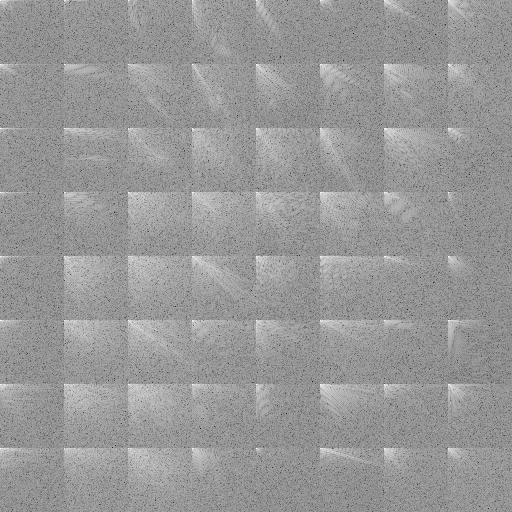
\includegraphics[width=0.8\textwidth]{dct_2d.png}
        \caption{2D DCT}
    \end{subfigure}
    \begin{subfigure}{0.32\textwidth}
        \centering
        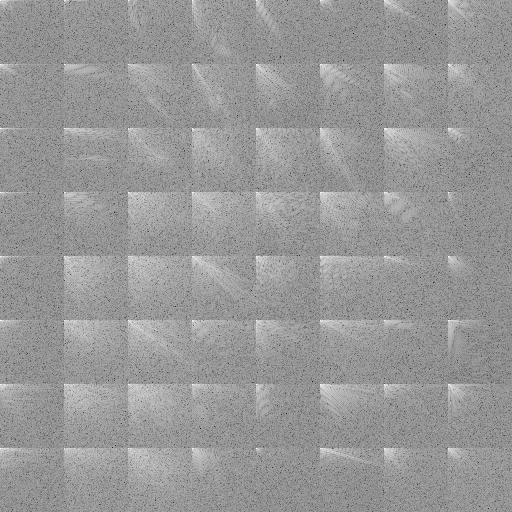
\includegraphics[width=0.8\textwidth]{dct_opencv.png}
        \caption{OpenCV DCT}
    \end{subfigure}
    \caption{coefficients in log domain}
\end{figure}

The following images are the result after performing IDCT.

\begin{figure}[H]
    \centering
    \begin{subfigure}{0.32\textwidth}
        \centering
        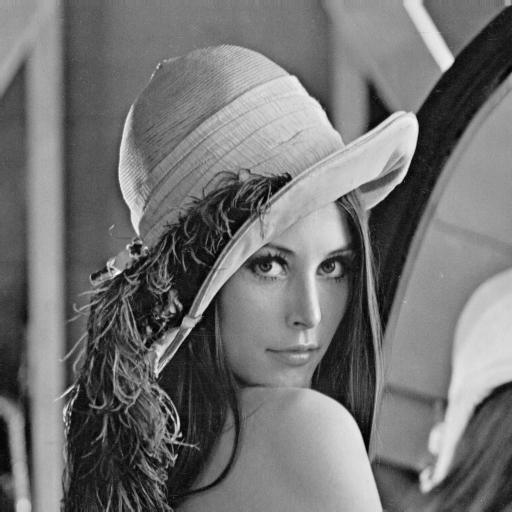
\includegraphics[width=0.8\textwidth]{idct_1d.png}
        \caption{Two 1D IDCT}
    \end{subfigure}
    \begin{subfigure}{0.32\textwidth}
        \centering
        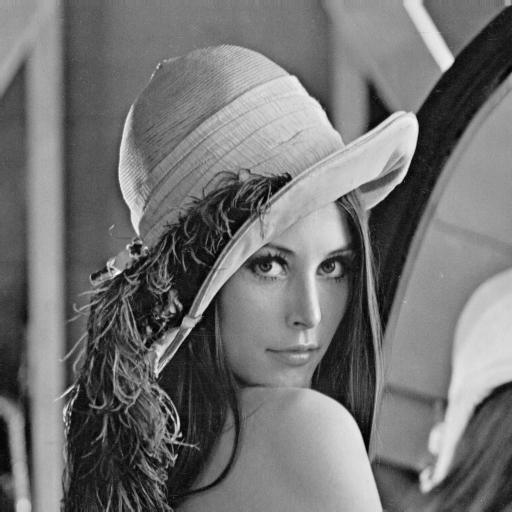
\includegraphics[width=0.8\textwidth]{idct_2d.png}
        \caption{2D IDCT}
    \end{subfigure}
    \begin{subfigure}{0.32\textwidth}
        \centering
        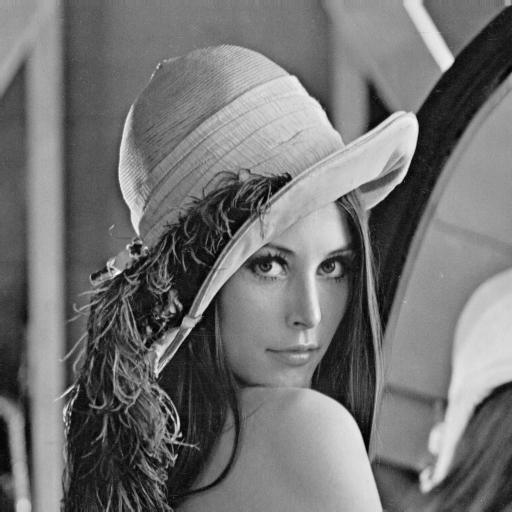
\includegraphics[width=0.8\textwidth]{idct_opencv.png}
        \caption{OpenCV IDCT}
    \end{subfigure}
    \caption{images after IDCT}
\end{figure}

The PSNR and runtime are as follows.

% Direct 2D-DCT time: 20.1545 seconds
% Two 1D-DCT time: 0.394455 seconds
% OpenCV DCT time: 0.00429717 seconds
% Direct 2D-IDCT time: 21.8392 seconds
% Two 1D-IDCT time: 0.436037 seconds
% OpenCV IDCT time: 0.00351246 seconds
% PSNR (Direct 2D-IDCT): 27.0035 dB
% PSNR (Two 1D-IDCT): 27.0035 dB
% PSNR (OpenCV IDCT): 27.0035 dB

\begin{table}[H]
    \centering
    \begin{tabular}{|c|c|c|c|}
        \hline
        Method & PSNR & Runtime(DCT) & Runtime(IDCT)  \\
        \hline
        2D DCT & \num{27.0035} & \num{20.1545} & \num{21.8392} \\
        Two 1D DCT & \num{27.0035} & \num{0.394455} & \num{0.436037} \\
        OpenCV DCT & \num{27.0035} & \num{0.00429717} & \num{0.00351246} \\
        \hline
    \end{tabular}
    \caption{PSNR and runtime}
\end{table}

\end{document}